\documentclass[numbers,handout]{ximera}
%% handout
%% nohints
%% newpage

\graphicspath{{./}{thePythagoreanTheorem/}{deMoivreSavesTheDay/}{complexNumbersFromDifferentAngles/}}

\usepackage{tikz}
\usepackage{tkz-euclide}
\usetkzobj{all}
\tikzstyle geometryDiagrams=[ultra thick,color=blue!50!black]
\newcommand{\tri}{\triangle}
\renewcommand{\l}{\ell}
\renewcommand{\P}{\mathcal{P}}
\newcommand{\R}{\mathbb{R}}
\newcommand{\Q}{\mathbb{Q}}

\newcommand{\Z}{\mathbb Z}

\renewcommand{\vec}{\mathbf}
\renewcommand{\d}{\,d}



%% Egyptian symbols

\usepackage{multido}
\newcommand{\egmil}[1]{\multido{\i=1+1}{#1}{
\includegraphics[scale=.1]{egyptian/egypt_person.pdf}\hspace{0.5mm}}}
\newcommand{\eghuntho}[1]{\multido{\i=1+1}{#1}{
\includegraphics[scale=.1]{egyptian/egypt_fish.pdf}\hspace{0.5mm}}}
\newcommand{\egtentho}[1]{\multido{\i=1+1}{#1}{
\includegraphics[scale=.1]{egyptian/egypt_finger.pdf}\hspace{0.5mm}}}
\newcommand{\egtho}[1]{\multido{\i=1+1}{#1}{
\includegraphics[scale=.1]{egyptian/egypt_lotus.pdf}\hspace{0.5mm}}}
\newcommand{\eghun}[1]{\multido{\i=1+1}{#1}{
\includegraphics[scale=.1]{egyptian/egypt_scroll.pdf}\hspace{0.5mm}}}
\newcommand{\egten}[1]{\multido{\i=1+1}{#1}{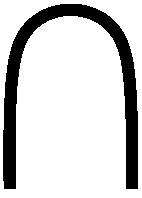
\includegraphics[scale=.1]{egyptian/egypt_heel.pdf}\hspace{0.5mm}}}
\newcommand{\egone}[1]{\multido{\i=1+1}{#1}{
\includegraphics[scale=.1]{egyptian/egypt_stroke.pdf}\hspace{0.5mm}}}
\newcommand{\egyptify}[7]{
 \multido{\i=1+1}{#1}{
\includegraphics[scale=.1]{egyptian/egypt_person.pdf}\hspace{0.5mm}}
 \multido{\i=1+1}{#2}{
\includegraphics[scale=.1]{egyptian/egypt_fish.pdf}\hspace{0.5mm}}
 \multido{\i=1+1}{#3}{
\includegraphics[scale=.1]{egyptian/egypt_finger.pdf}\hspace{0.5mm}}
 \multido{\i=1+1}{#4}{
\includegraphics[scale=.1]{egyptian/egypt_lotus.pdf}\hspace{0.5mm}}
 \multido{\i=1+1}{#5}{
\includegraphics[scale=.1]{egyptian/egypt_scroll.pdf}\hspace{0.5mm}}
 \multido{\i=1+1}{#6}{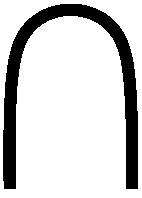
\includegraphics[scale=.1]{egyptian/egypt_heel.pdf}\hspace{0.5mm}}
 \multido{\i=1+1}{#7}{
\includegraphics[scale=.1]{egyptian/egypt_stroke.pdf}\hspace{0.5mm}}
 \hspace{.5mm}
}




\let\masterdocument\document
\let\endmasterdocument\enddocument
\let\masterinput\input



\begin{masterdocument}
\begin{titlepage}
    \vspace*{1in}
    \begin{center}
      {\Huge \bfseries History of mathematics}\\[0.5cm]
      {\Large Bart Snapp}\\[0.4cm]
      This document was typeset on \today.
    \end{center}
    %\vspace*{\fill}
  \end{titlepage}

\setcounter{page}{2}

\tableofcontents

\renewcommand{\documentclass}{\setbox0\vbox}
\renewcommand{\input}{\setbox0\vbox}
\renewenvironment{document}{}{}

\masterinput{./whatIsANumber/whatIsANumber.tex}
\masterinput{./measuringWithFractions/measuringWithFractions.tex}
\masterinput{./theMethodOfFalsePosition/theMethodOfFalsePosition.tex}
\masterinput{./babylonianNumbers/babylonianNumbers.tex}
\masterinput{./rationalNumbersAndSimilarity/rationalNumbersAndSimilarity.tex}
\masterinput{./pythagoreanMeans/pythagoreanMeans.tex}
\masterinput{./computingQuadratures/computingQuadratures.tex}
\masterinput{./squaringTheCircleWithLunes/squaringTheCircleWithLunes.tex}
\masterinput{./euclidsElements/euclidsElements.tex}
\masterinput{./trianglesOnACone/trianglesOnACone.tex}
\masterinput{./thePythagoreanTheorem/thePythagoreanTheorem.tex}
\masterinput{./theUniqueFactorizationTheorem/theUniqueFactorizationTheorem.tex}
\masterinput{./heronsFormula/heronsFormula.tex}
\masterinput{./solvingEquations/solvingEquations.tex}
\masterinput{./complexNumbersFromDifferentAngles/complexNumbersFromDifferentAngles.tex}
\masterinput{./deMoivreSavesTheDay/deMoivreSavesTheDay.tex}
\masterinput{./theBinomialTheoremAndPi/theBinomialTheoremAndPi.tex}
\masterinput{./newtonAndKepler/newtonAndKepler.tex}
\masterinput{./leibnizAndSeries/leibnizAndSeries.tex}
\masterinput{./bernoulliEulerAndSeries/bernoulliEulerAndSeries.tex}
\masterinput{./cantorCan/cantorCan.tex}
\masterinput{./theFoundationsOfGeometry/theFoundationsOfGeometry.tex}
\masterinput{./cityGeometry/cityGeometry.tex}

\end{masterdocument}
